\section*{Scenario-I : Fitting Circle}
\vspace*{-.2cm}
The following figures(\ref{circ},\ref{line}) illustrate two circular models approximated for the points depicted by dots. With proper tuning of the threshold, parameters of first model(\ref{circ},R=9.856 \& O$\equiv$[0.123,-0.156]) stays closer to the parameters of the circle used to create half of these noisy points(R=10 \& O$\equiv$[0,0]). The second model(\ref{line}) seems to depict the nature of noisy line used to create half the data points.
\begin{figure}[h]
    \begin{minipage}{.48\textwidth}
        \begin{center}
            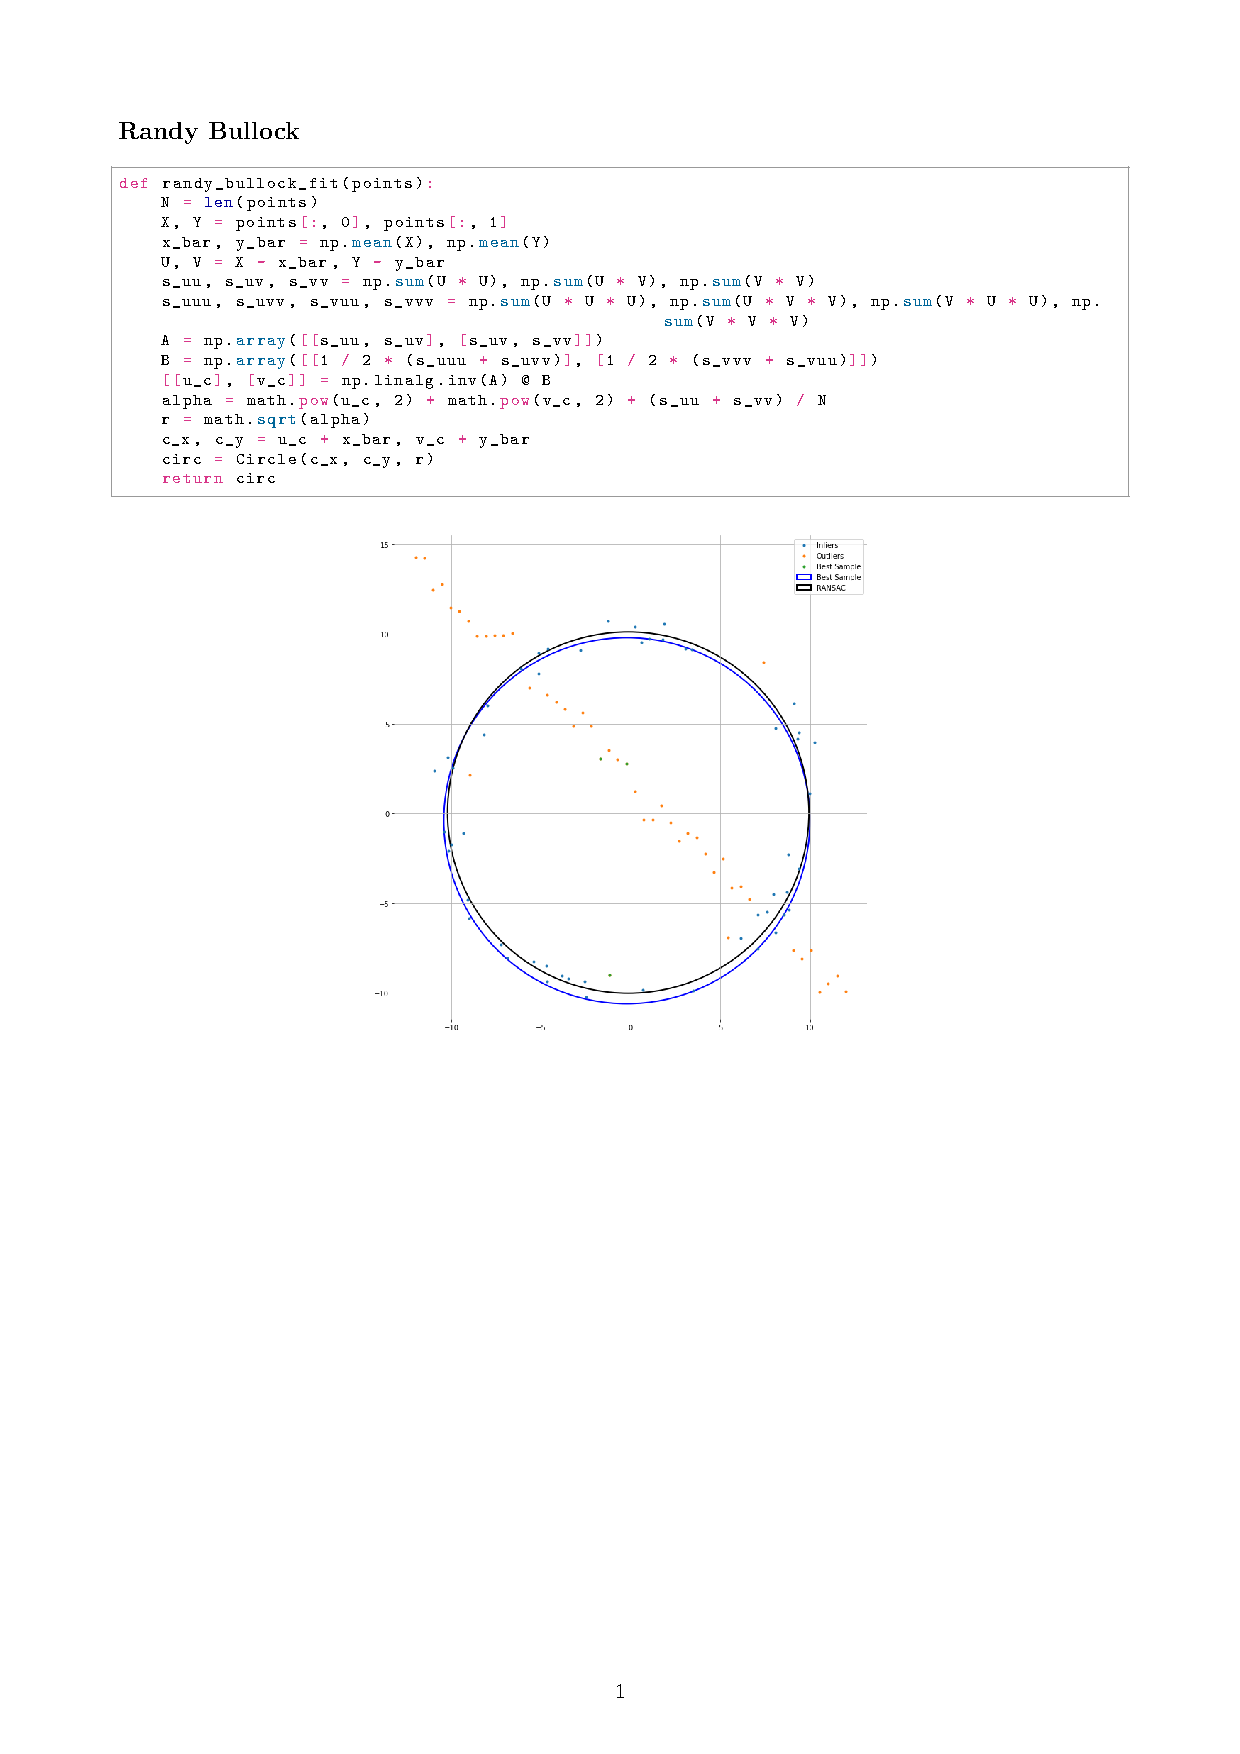
\includegraphics[width=.75\columnwidth]{circle}
            \caption{Model I}
            \label{circ}
        \end{center}
    \end{minipage}
    \begin{minipage}{.48\textwidth}
        \begin{center}
            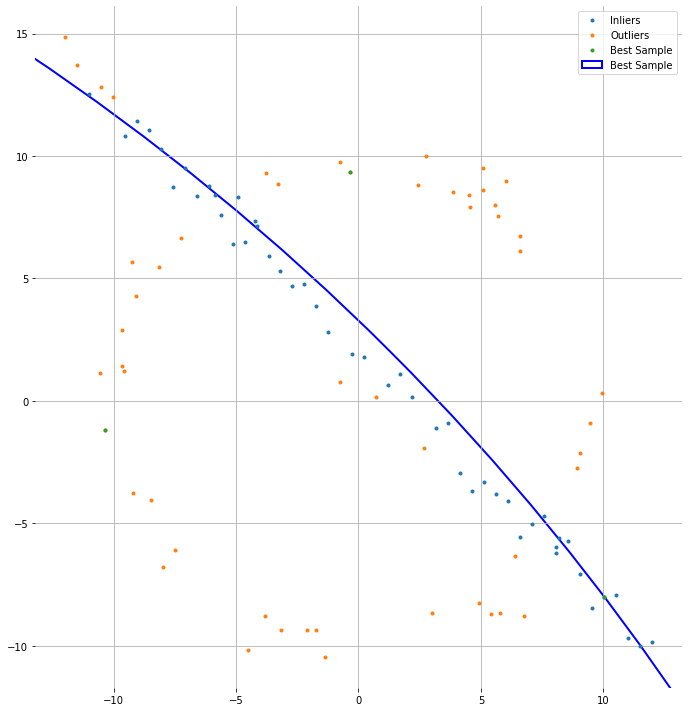
\includegraphics[width=.75\columnwidth]{line}
            \caption{Model II}
            \label{line}
        \end{center}
    \end{minipage}
\end{figure}
\newpage
\section*{Scenario-II : Fitting Homography}
The following figures show the transformation of the Graffiti \textit{im1.ppm} onto \textit{im5.ppm} using the provided homography. Consider the area enclosed using the green-colored bounding box. The transition between two images is almost indistinct and it will be completely seamless if the intenseness of the pixels around the transitions are accurately matched.
\begin{figure}[h]
    \begin{center}
        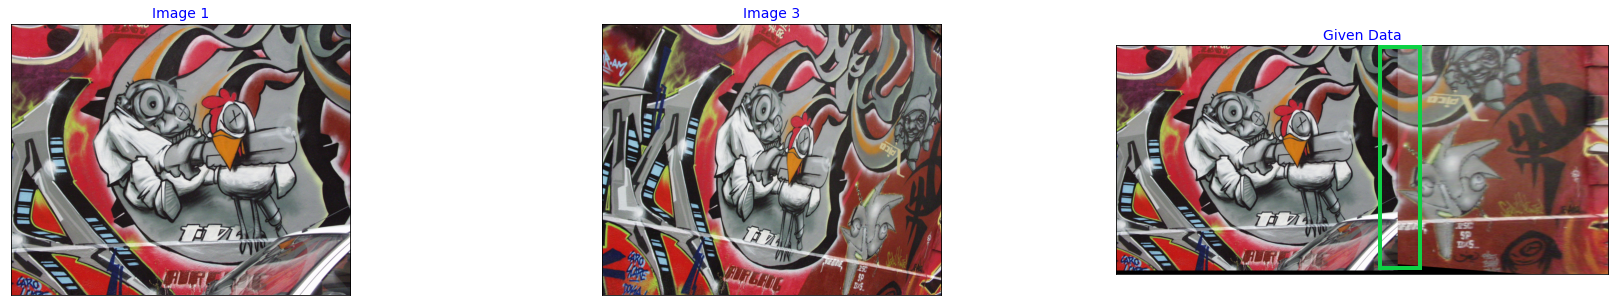
\includegraphics[width=\columnwidth]{q3_1}
    \end{center}
\end{figure}
\\
The following illustration shows the same stitching using the homography extracted from a RANSAC implementation. Firstly the matching features between two images are extracted using the SIFT feature. Then these features are matched using a RANSAC execution with proper thresholding to achieve the transformation homography.
\begin{figure}[h]
    \begin{center}
        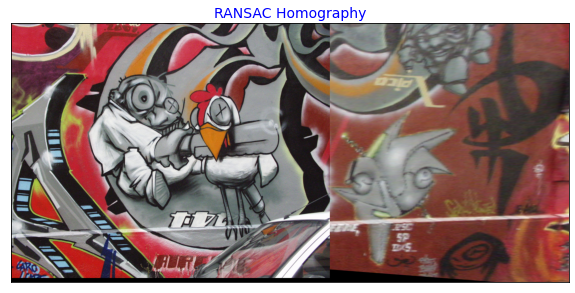
\includegraphics[width=.75\columnwidth]{q3_2}
    \end{center}
\end{figure}
\\
Direct matching between the two images doesn't seem to work due to the scarcity of good matching feature count. Hence it is decided to match adjacent figures(img1 \& img2, img2 \& img3....) which are having more than 1000 matches. And deriving the overall transformation by multiplying adjacent ones. Although a slight translation is visible inside the green bounding box the result can be regarded as a tighter extraction for a basic implementation.
$$H_{1\to5}=H_{4\to5}\cdot H_{3\to4}\cdot H_{2\to3}\cdot H_{1\to2}$$
\vspace*{.2cm}
\begin{minipage}{.48\textwidth}
    \begin{equation*}
        H_{given}=\begin{bmatrix}
            0.625 & 0.058 & 222.012 \\
            0.222 & 1.165 & -25.606 \\
            0.001 & 0.000 & 1.000
        \end{bmatrix}
    \end{equation*}

\end{minipage}
\begin{minipage}{.48\textwidth}
    \begin{equation*}
        H_{ransac}=\begin{bmatrix}
            0.594 & 0.023 & 227.644 \\
            0.215 & 1.066 & -8.788  \\
            0.001 & 0.000 & 1.000
        \end{bmatrix}
    \end{equation*}
\end{minipage}
\section*{References}
\begin{enumerate}
    \item \href{https://dtcenter.org/sites/default/files/community-code/met/docs/write-ups/circle_fit.pdf}{Randy Bullock Fit}
    \item \href{https://docs.opencv.org/4.x/}{opencv}
    \item \href{https://sdg002.github.io/ransac-circle/index.html}{An article about implementation of RANSAC for circle fitting.}
    \item \href{https://programmer.group/panoramic-stitching-using-ransac-algorithm.html}{Panoramic stitching using RANSAC algorithm}
    \item \href{https://youtu.be/J1DwQzab6Jg}{Youtube playlist on Image Stitching}
\end{enumerate}
\vspace*{.8cm}
\HRule
\vspace*{-.2cm}
\begin{center}
    Executable code for the assignment can be found \href{https://github.com/sanjith1999/EN2550-Assignments/tree/master/Fitting%20and%20Alignment}{here}
\end{center}